\chapter{Review of related software libraries}
\label{chapt:technology}
In this chapter, we review some software libraries that can be used for implementing the algorithms required for constructing a destructible environment. We do not talk about all-in-one software development kits with their approach to a destructible environment already implemented. Instead, our focus is on building a game with our own approach to the destructible environment. 

To build a game, we will surely need a physics engine, a graphics engine, and a selection of geometric libraries to support the computation of the destructible environment. We mention which libraries we used in the implementation and details of their use can be found in~\cref{app:implementation}.

\section{Physics engine}
\label{sec:phyengine}
Physics engines are used in games to provide a simulation of applied forces to in-game objects and collision detection. Many physics engines are directly bundled with rendering, audio engines to create a complete game engine. 

To support our implementation of destructible environment we need a physics engine to detect collisions, move the user-controlled vehicle and simulate gravity and mechanical forces. There are no special needs for the physics engine in our applications that would not be supported in most engines. Some of the commonly used engines are Open Dynamics Engine, Newton Game Dynamics, Bullet, Simulation Open Framework Architecture, Tokamak. All of them provide the simulation of rigid bodies and collision detection. Other features are not relevant to us. Therefore we decided to used Bullet physics on the base of author's previous experience.

\section{Geometric libraries}
Here we preview some of the libraries focused on a decomposition or modification of 3D meshed objects. The preview is focused on three techniques used in destructible environment, boolean operations, Voronoi tessellation and convex decomposition,

\subsection{Boolean operations}
When searching for efficient library able to compute the difference of two 3D triangular meshes, we found out that the majority of available software
is dependent on using \textbf{The Computational Geometry Algorithms Library}~\footnote{\url{http://www.cgal.org/}} or shortly \textbf{CGAL}. CGAL provides polyhedral surfaces that are closed for Boolean operations, and it is possible to convert data between meshes and polyhedrons. 

The mentioned polyhedral surfaces or Nef polyhedrons~\cite{nefpoly}, require the input mesh to be an orientable 2-manifold (for more details on this data structure see~\cref{app:implementation}). Nef polyhedron works with two data structures, one that represents the local neighborhoods of vertices, which is in itself already a complete description, and a data structure that connects these neighborhoods up to a global data structure with edges, facets, and volumes. This redundancy in data makes Nef polyhedron a large data structure that is not optimized for fast construction and not the most suitable for real-time deployment.

We also considered using a \textbf{Cork Boolean Library}~\footnote{\url{https://github.com/gilbo/cork\#cork-boolean-library}} but we did not find it to be as robust as CGAL and encountered problems and instability on valid data.

\subsection{Voronoi tessellation}
We learned that to Voronoi tessellation can be beneficial to either creating a compound body held together by springs or used as a tool for subtracting parts of the mesh. Here are some libraries useful for both tasks.

\begin{description}
\item[CGAL] also includes package providing different 3D triangulations, mainly Delaunay triangulation and the possibility of creating Voronoi diagram as its dual graph. However, CGAL does not provide means to clip the Voronoi cells against the surface mesh.

\item[Voro++]~\footnote{\url{http://math.lbl.gov/voro++/}} is a library for carrying out three-dimensional computations of the Voronoi tessellation. It calculates Voronoi cell for each particle individually and is suited for high-performance calculations on large scale particle systems. It is also able to clip Voronoi cells to any user defined boundary. This library would be well suited for decomposing entire objects into Voronoi cells. 

\item[Qhull]~\footnote{\url{http://www.qhull.org/}} provides the means to compute convex hull, Delaunay triangulation, Voronoi diagram in 2,3 or 4 dimensional space.

\end{description}
Because implementation requires only one Voronoi cell per collision, we chose to use the simpler Voro++ library for this task. 


\subsection{Convex decomposition}
\label{sec:decompositionLib}
Convex decomposition is critical to fast and accurate collision detection on 3D meshes. We introduce two libraries with different approaches to the task.
\begin{description}
\item[CGAL] provides the means for decomposing the polyhedral shape (triangular mesh can be converted into polyhedron) into a set of convex polyhedrons. CGAL is aiming for an exact convex decomposition, which produces a large number of small pieces~\footnote{\url{http://doc.cgal.org/latest/Convex\_decomposition\_3}}.

\item[Hierarchical Approximate Convex Decomposition] or HACD~\cite{HACD} is a library and algorithm providing a convex decomposition that approximates the original shape. The approximation yields fewer pieces and is faster than exact calculations, but the result is not exact. For the reasons that we are implementing a destructible environment in a computer game, we can allow for deviations in the shape of the objects from their respective visual representations. Those deviations should be too small to be noticed in the game. This makes us choose HACD over CGAL.

\item[Convex Decomposition Library]~\footnote{\scriptsize\url{http://codesuppository.blogspot.cz/2009/11/convex-decomposition-library-now.html}} produces approximate convex decomposition. It is an older library that is currently marked deprecated in favor of HACD. 
\end{description}

We can see the difference in the result of exact and approximate approaches on~\cref{fig:bunny}. It is evident that we do not want to use the exact decomposition in a computer game, but on the other hand for the simulations where the calculation time is not critical, the approximations should not be used.
\begin{figure}
        \centering
        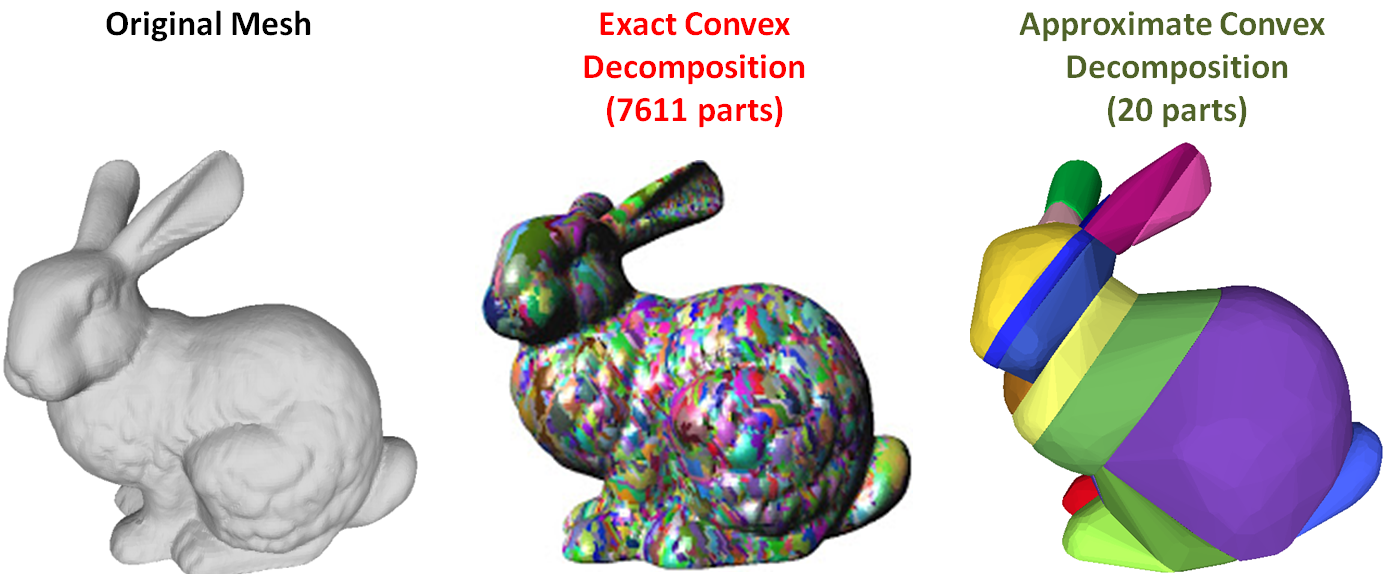
\includegraphics[width=\textwidth]{img/bunny}
        \caption{Difference between original mesh, exact convex decomposition and an approximate convex decomposition. Source: \url{https://github.com/kmammou/v-hacd}}
        \label{fig:bunny}
\end{figure}


